\section{RCRRTExt\-Ext  Class Reference}
\label{classRCRRTExtExt}\index{RCRRTExtExt@{RCRRTExt\-Ext}}
Dual tree version of {\bf RCRRT} {\rm (p.\,\pageref{classRCRRT})} with Ext\-Ext method, which is used to do experiments with spacecraft model in 3D grid environment considering the dynamic constraints . 


{\tt \#include $<$rcrrt.h$>$}

Inheritance diagram for RCRRTExt\-Ext::\begin{figure}[H]
\begin{center}
\leavevmode
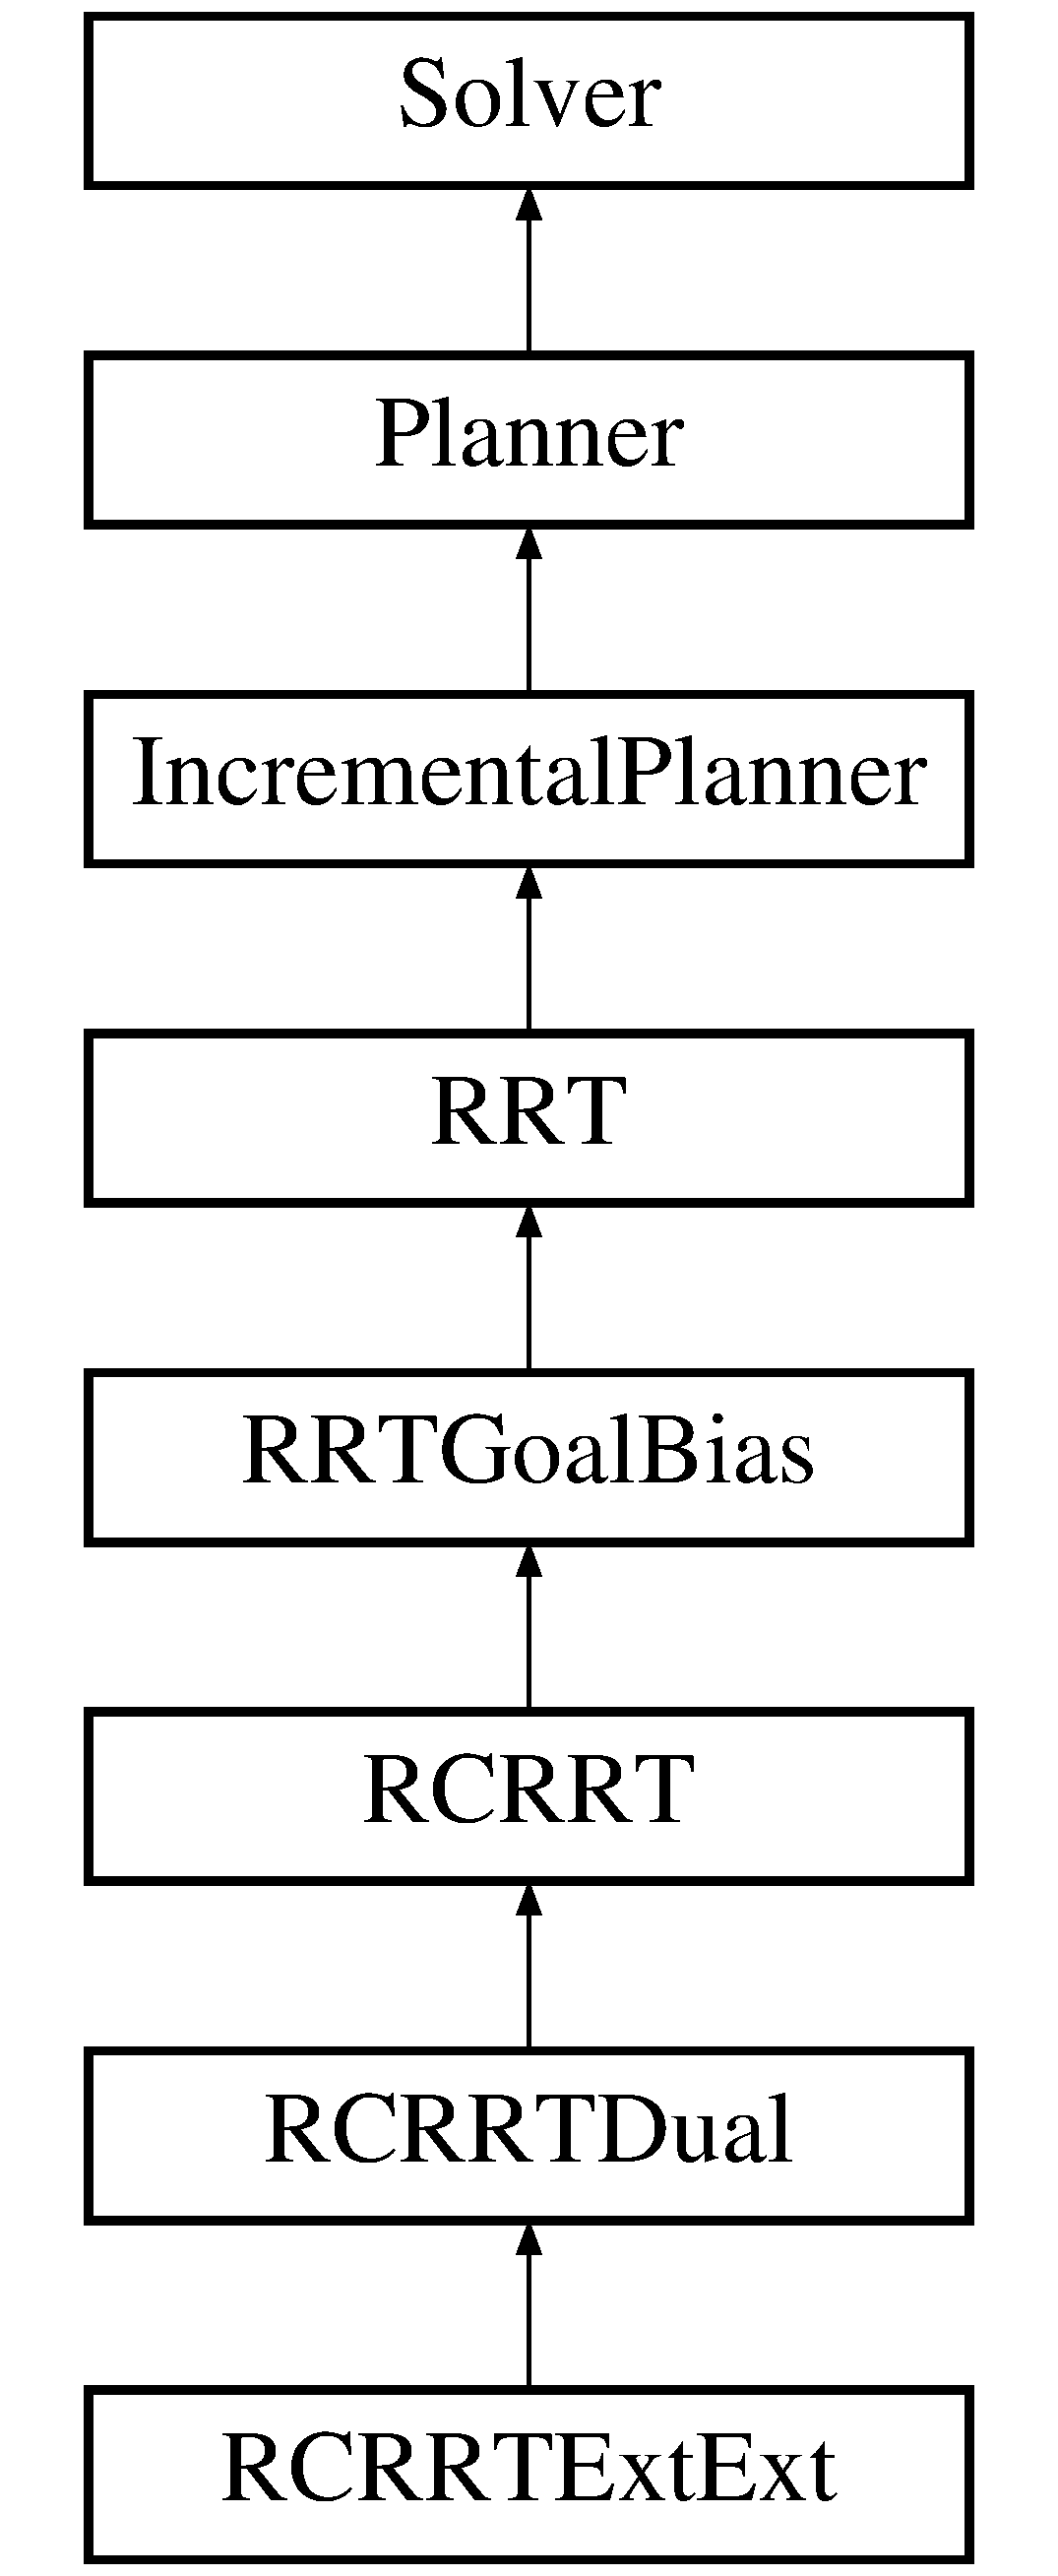
\includegraphics[height=8cm]{classRCRRTExtExt}
\end{center}
\end{figure}
\subsection*{Public Methods}
\begin{CompactItemize}
\item 
{\bf RCRRTExt\-Ext} ({\bf Problem} $\ast$p)
\item 
virtual {\bf $\sim$RCRRTExt\-Ext} ()
\item 
virtual bool {\bf Plan} ()
\begin{CompactList}\small\item\em Attempt to solve an Initial-Goal query by growing an {\bf RRT} {\rm (p.\,\pageref{classRRT})}.\item\end{CompactList}\end{CompactItemize}


\subsection{Detailed Description}
Dual tree version of {\bf RCRRT} {\rm (p.\,\pageref{classRCRRT})} with Ext\-Ext method, which is used to do experiments with spacecraft model in 3D grid environment considering the dynamic constraints .



\subsection{Constructor \& Destructor Documentation}
\index{RCRRTExtExt@{RCRRTExt\-Ext}!RCRRTExtExt@{RCRRTExtExt}}
\index{RCRRTExtExt@{RCRRTExtExt}!RCRRTExtExt@{RCRRTExt\-Ext}}
\subsubsection{\setlength{\rightskip}{0pt plus 5cm}RCRRTExt\-Ext::RCRRTExt\-Ext ({\bf Problem} $\ast$ {\em p})}\label{classRCRRTExtExt_a0}


\index{RCRRTExtExt@{RCRRTExt\-Ext}!~RCRRTExtExt@{$\sim$RCRRTExtExt}}
\index{~RCRRTExtExt@{$\sim$RCRRTExtExt}!RCRRTExtExt@{RCRRTExt\-Ext}}
\subsubsection{\setlength{\rightskip}{0pt plus 5cm}virtual RCRRTExt\-Ext::$\sim$RCRRTExt\-Ext ()\hspace{0.3cm}{\tt  [inline, virtual]}}\label{classRCRRTExtExt_a1}




\subsection{Member Function Documentation}
\index{RCRRTExtExt@{RCRRTExt\-Ext}!Plan@{Plan}}
\index{Plan@{Plan}!RCRRTExtExt@{RCRRTExt\-Ext}}
\subsubsection{\setlength{\rightskip}{0pt plus 5cm}bool RCRRTExt\-Ext::Plan ()\hspace{0.3cm}{\tt  [virtual]}}\label{classRCRRTExtExt_a2}


Attempt to solve an Initial-Goal query by growing an {\bf RRT} {\rm (p.\,\pageref{classRRT})}.



Reimplemented from {\bf RCRRTDual} {\rm (p.\,\pageref{classRCRRTDual_a2})}.

The documentation for this class was generated from the following files:\begin{CompactItemize}
\item 
{\bf rcrrt.h}\item 
{\bf rcrrt.C}\end{CompactItemize}
